\documentclass[10pt,a4paper]{report}
\usepackage[latin1]{inputenc}
\usepackage{amsmath}
\usepackage{amsfonts}
\usepackage{amssymb}
\usepackage{graphicx}
\usepackage{siunitx}
\usepackage{hyperref}

\begin{document}
\newpage


\section{Average Decay Length of Kaon}


To estimate the average decay length of the kaon we used the data of an other experiment named LifeK, which was using the same beam line and the same beam momentum as the K2Pi experiment. In the LifeK experiment the beam was composed of $84\%$ positively charged pions $\pi^+$ and $16\%$ kaons $K^+$. In total there are $100`000$ measurements of decay lengths of the particles. This means the data from the LifeK experiment corresponds to a convolution of two exponential distributions with the parameters $\tau_{\pi^+}$ and $\tau_{K^+}$, the average decay length of the two particle, and two normalization constants, which correspond to the number of each particle. The probability for a kaon to decay at the point x is given by the following equation.

\begin{equation}
\label{convolutedDistribution}
P(x)=  \frac{n_{\pi^+}}{\tau_{\pi^+}} \cdot e^{-x/ \tau_{pi^+}} + \frac{n_{K^+}}{\tau_{K^+}} \cdot e^{-x/ \tau_{K^+}}
\end{equation} 
We already know three of those parameters:
\begin{align*}
n_{\pi^+} &= 84`000 \\
n_{K^+} &= 16`000 \\
\tau_{\pi^+} &= 4188 m
\end{align*}

To find the average decay length of the kaon we tried two different methods.\\
First, we estimated $\tau_{K^+}$ directly from the given data with the scipy.optimizer.curvefit where we fitted the function given by equation \ref{convolutedDistribution}. We left all four parameters of the equation as independent variables, but initialised them at the expected value, and bound them in reasonable bounds. In order to have an idea what to expect for the average decay length of the kaon we calculated the average decay length $\tau_{K^+}= \gamma \beta \omega_{K^+}$ where $\omega_{K^+}$ is the mean lifetime of the kaon which is $(1.2379 \pm 0.0021) \times 10^{-8} s $ accordig to the particle data group (\url{http://pdg.lbl.gov/2016/listings/rpp2016-list-K-plus-minus.pdf}, Page 2, 2016) For the expected value of the kaon we get $563.7 m$

This method leads to this result:\\
\\

\begin{tabular}{c|cc}
 & Estimated Value  & Uncertainty \\ 
\hline 
$\hat{\tau}_{K^+}$ & 577 m & 6 m \\ 

$\hat{\tau}_{\pi^+}$ & 41890 m  & 21 m  \\

${n_{\pi^+}}/{n_{K^+}}$ & 0.697 & 0.0066 \\ 

$n_{K^+}$ & 12375 & 63 \\
\end{tabular} 

In comparison to the expected value of $563.7 m$ the estimated $\tau_{K^+}$ is quite good. But because all other parameters are independent, they are different to our assumption.
\\
\\
For the second method to estimate $\tau_{K^+}$ we separated the two exponential distribution using Monte Carlo Method to simplify the fit function. We represented the data of LifeK in a histogram with 100 bins. We simulated an exponential distribution with the scale of $\tau_{\pi^+}$ and represented the simulated data in a histogram, using the same bins as before. We subtracted the values of the two histograms to get the distribution of the kaon. To estimate the average decay length we use Maximum-Likelihood Method. To estimate the uncertainty we repeat the Maximum-Likelihood Method N (=1`000) times to calculate the mean value of $\hat{\tau}_{K^+}$. The uncertainty $m_{\tau}$ then can be determined using the standard deviation $\sigma_{\hat{\tau}}$.

\begin{align*}
\hat{\tau}_{K^+}&= \frac{\sum_{i=1}^{100} (x_i \cdot n_i)}{\sum_{i=1}^{100} n_i}\\
m_{\hat{\tau}}&= \frac{\sigma_{\hat{\tau}}}{\sqrt{N}}
\end{align*}
The results are:
\begin{align*}
\hat{\tau}_{K^+}&=578.x m \\
m_{\hat{\tau}}&=2.4 m
\end{align*}


\begin{figure}[htbp] 
  \centering
     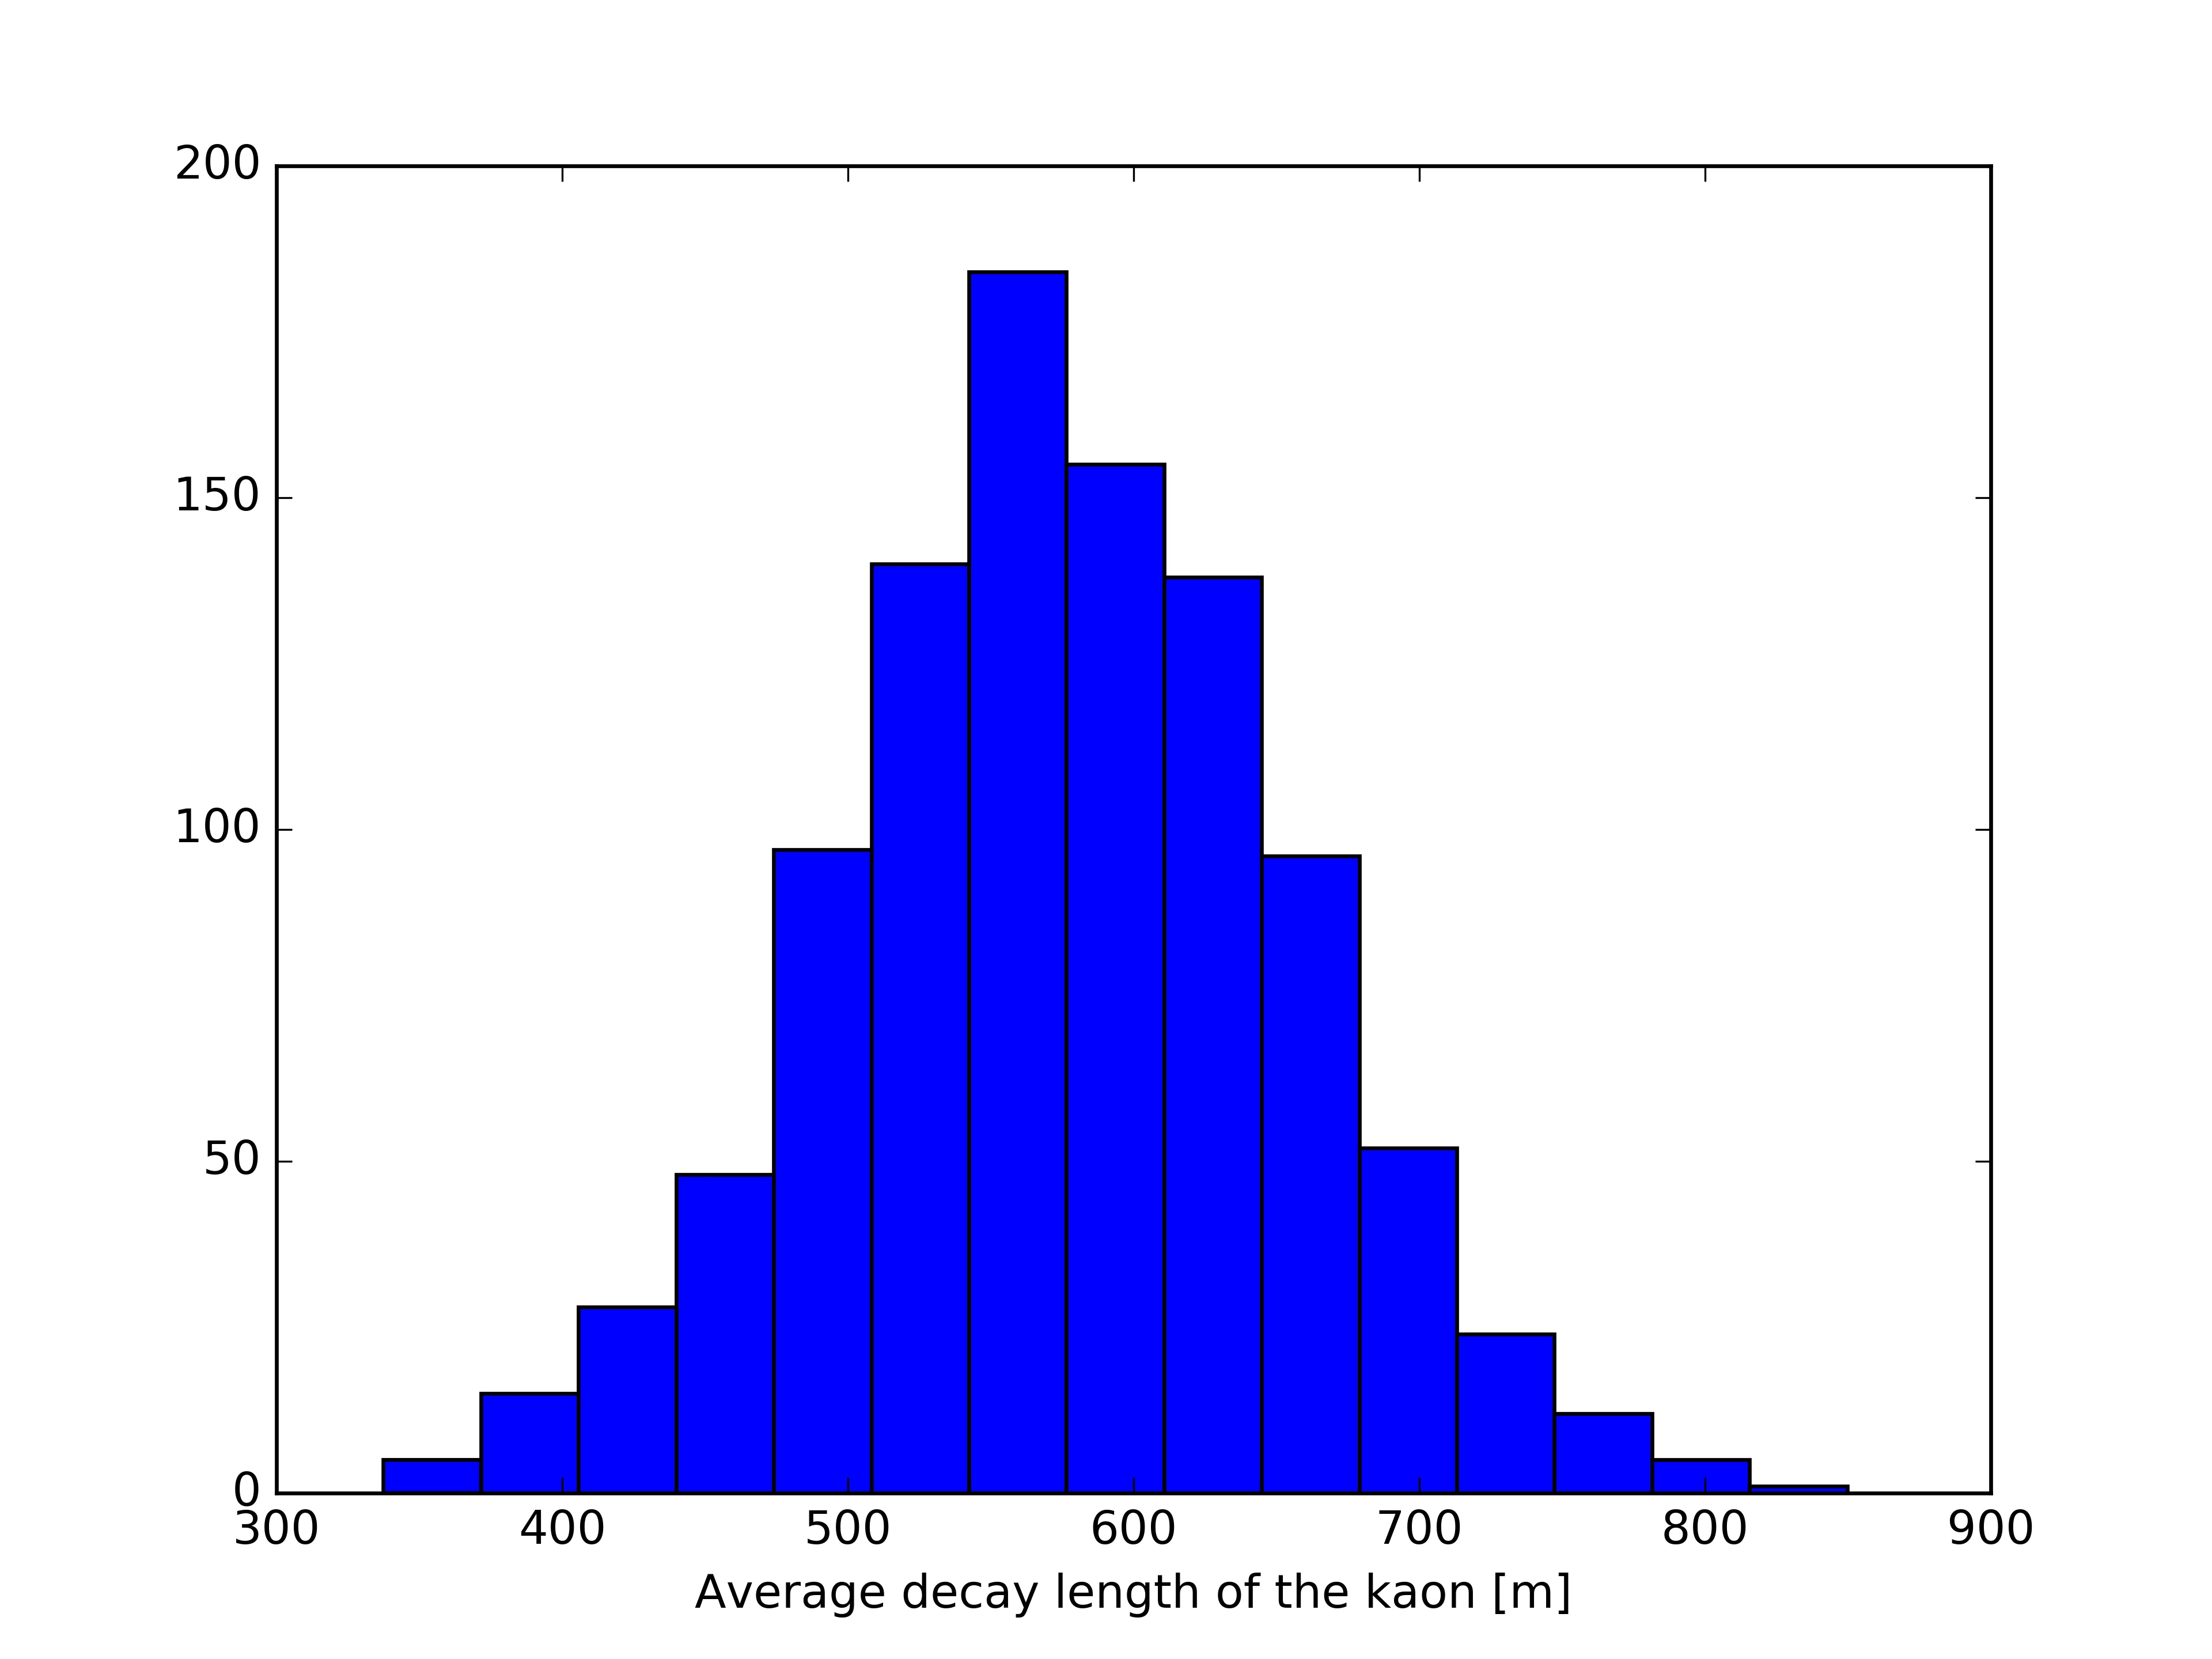
\includegraphics[width=0.7\textwidth]{hist_tau_estimator3.jpg}
  \caption{Gaussian distribution of $\hat{\tau}_{K^+}$ estimator}
  \label{fig:Bild1}
\end{figure}

We decided to use the results of the second method because of the following reasons. The uncertainty of the second method is smaller. With the first method we used e predefined function, where we did not understand exactly what was calculated, whereas with the second method we understood every step. Thirdly, we could not explain the change of the independent variables. 
\end{document}